% res_carry.tex -- Results 4.1: carrying with a fixed team (RQ1), rig twin and rig side by side.
% 17 Oct (v3_full): rebuilt on the freeze results. The twin carry is the claim of card
% docs/experiments/2026-10-16_carry_speed_envelope.md (bars frozen 16 Oct 08:05; R1847-R1886; reviewer SUPPORTED WITH
% CORRECTIONS, its must-not-say list honoured: no "path-tracking RMSE" or "tilt during the carry" for the frozen
% columns, no trend read from the peak-tilt column, "peak path speed", the 1 m arm's window caveat). The clock-free
% columns (cut, across-path rms, lag, path-window tilt) are reported, not scored (Wesley 16 Oct): tools/corner_metrics.py
% R1847-R1886, 16 Oct 17:32; the 0.3 m/s base rows also in docs/experiments/2026-10-16_corner_cutting.md. The rig carry
% (T7) is skel_carry's table on the reviewer's window (12 Oct). The landing paragraph: appendix re-fly (C-L1 NOT
% supported, the reviewer's false touchdown) and card 2026-10-17_touchdown_height_gate (A: twin default; rig after
% the critic). fig:flight and fig:traj are the 17 Oct re-renders on the freeze tree (R2034; R1853, R1849).

\subsection{Carrying with a fixed team}
\label{sec:res_carry}

This section answers RQ1: what does feeding the trackers the rod pull they measure buy, and which sources of steady
payload error remain? It first establishes the carry itself, in the rig twin over a speed envelope and on the rig on
the two paths it flew, then the steady errors. The twin's baseline is its own cell at 0.125\,m/s, the speed the rig
has flown; the rig's is the same path flown that morning on the planner's pull. The bars are the carry card's,
frozen before its runs. This carry is in turn the baseline for RQ2 and RQ3.

\subsubsection{Takeoff and lift}

Figure~\ref{fig:flight} shows one whole flight of the rig twin with the default controller: the rod sweep, the
pretension, the lift, a hold at 1.0\,m and LAND (Section~\ref{sec:takeoff}).

\begin{figure}[h]
\centering
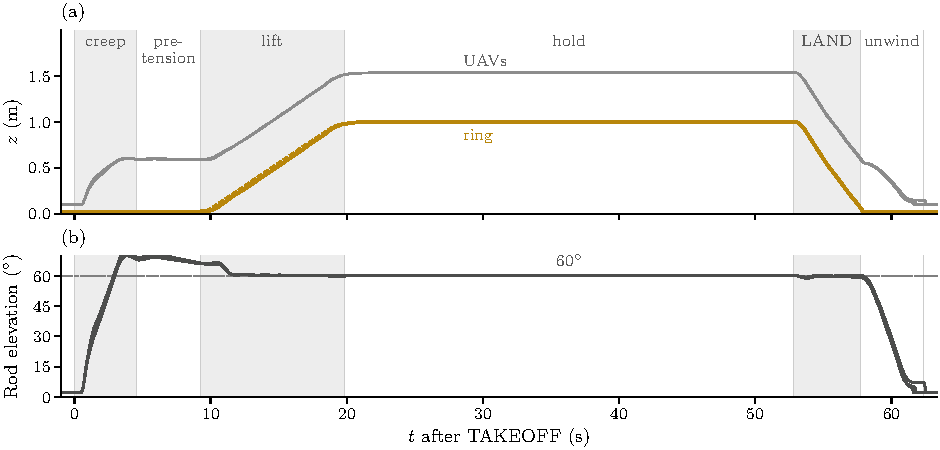
\includegraphics[width=\textwidth]{Images/flight.pdf}
\caption[One flight from the floor]{One flight from the floor in the rig twin: three carriers, hover at 1.0\,m, the
default controller (their traces overlap). (a) Heights of the ring (gold; dashed: its planned height) and of the
UAVs (grey); shaded: the creep, the lift and LAND. (b) Elevation of each rod above the horizontal; dotted: the
planned 60$^\circ$. In the creep the UAVs climb and swing their rods up from the floor, past the planned elevation,
without lifting the ring; in the pretension they hold their height while the rod feedforward eases in; the ring
then leaves the floor and follows its lift ramp to 1.0\,m while the rods settle on 60$^\circ$. On LAND the ring and
the UAVs descend together until the ring is on the floor; the UAVs then unwind along their rods.}
\label{fig:flight}
\end{figure}

\subsubsection{The carry in the twin: a speed envelope}
\label{sec:res_envelope}

Table~\ref{tab:T7t} gives the three-carrier carry in the rig twin: five load paths at three peak path speeds, two
runs per cell on one code tree, and an arm with 1\,m cables, scored against four bars frozen before the runs: no
abort, drop or unannounced detach, with every UAV landed and disarmed; a ring RMSE of at most 25\,mm (from 5\,s after TAKEOFF to LAND, lift and landing included); a peak ring
tilt of at most 6$^\circ$; and a radius ratio of at least 0.95. 39 of the 40 runs pass every bar. The spin at
0.3\,m/s fails the tilt bar once (6.31$^\circ$, mid-spin; its repeat 3.76$^\circ$), so as frozen that cell is outside
the envelope, and it was not re-flown; every other cell is inside at 0.125, 0.2 and 0.3\,m/s. The radius ratio lies
between 0.966 and 1.004 over all 40 runs (for the line, the ratio of amplitudes about its centre). The 1\,m cables
pass every bar, with a ring RMSE at most 1.27 times their 0.55\,m cell's mean on the frozen window (1.35 times on the
path alone); their configurations also land 5\,s later, so the comparison is not one variable.

\begin{table}[htbp]
\centering
\footnotesize
\setlength{\tabcolsep}{2.6pt}
\caption[The carry in the twin: the speed envelope]{The three-carrier carry in the rig twin: 0.86\,kg ring at
1.0\,m on 0.55\,m rods (lower block: 1\,m cables), floor start, the default controller, two runs per cell on one
code tree; each cell gives the range over its two runs. Scored against the bars frozen before the runs: the ring RMSE
from 5\,s after TAKEOFF to LAND, lift-off, hovers and descent included, against the planner's 10\,Hz held reference
(bar 25\,mm), and the peak ring tilt over the whole flight, lift-off and landing included (bar 6$^\circ$). Reported
beside them, not scored: the same RMSE and the peak tilt over the path alone, and the clock-free measures of
Section~\ref{sec:metrics}: the cut (mean distance inside the path over its tightest quarter), the across-path rms over
the fast part of the path, and the lag behind the schedule (+ late). Speed: the peak path speed. $^a$\,One run over the
tilt bar: the cell is outside the envelope. Line: no curvature, so no cut; its lag is not defined at the turns and is
not given.}
\label{tab:T7t}
\begin{tabular}{llccccccc}
\toprule
 & & \multicolumn{2}{c}{Scored} & \multicolumn{5}{c}{Reported} \\
\cmidrule(lr){3-4}\cmidrule(lr){5-9}
 & Speed & Ring RMSE & Peak tilt & Path RMSE & Path tilt & Cut & Across rms & Lag \\
Path & (m/s) & (mm) & ($^\circ$) & (mm) & ($^\circ$) & (mm) & (mm) & (ms) \\
\midrule
Circle & 0.125 & 8.8--10.6 & 1.8--1.9 & 4.3 & 0.9--1.1 & 2.4--2.5 & 2.7--2.8 & 55--70 \\
 & 0.2 & 9.2--12.4 & 1.7 & 6.2--8.9 & 1.4--1.6 & 3.4--6.6 & 4.4--8.3 & 32--73 \\
 & 0.3 & 14.0--14.7 & 2.0--2.8 & 13.4--14.3 & 2.0--2.8 & 13.0--14.3 & 14.6--15.8 & 54--56 \\
\addlinespace
Figure-eight & 0.125 & 10.3--12.7 & 2.3 & 6.0--8.9 & 1.0--1.1 & 4.9--10.0 & 3.5--7.1 & 34--63 \\
 & 0.2 & 13.6--14.5 & 1.9--2.0 & 11.9--12.4 & 1.5--1.7 & 15.8--16.0 & 10.2--10.9 & 36--44 \\
 & 0.3 & 17.8--17.9 & 2.3--2.4 & 20.2--20.9 & 2.3 & 28.5--31.1 & 17.9--20.6 & 15--25 \\
\addlinespace
Line & 0.125 & 6.5--8.3 & 1.9--2.0 & 4.3--5.3 & 0.9--1.0 & -- & 0.4--0.5 & -- \\
 & 0.2 & 9.1--9.8 & 2.5--2.8 & 8.3--9.0 & 1.5--1.9 & -- & 0.5--1.1 & -- \\
 & 0.3 & 12.5--16.8 & 3.0--3.7 & 12.9--16.9 & 2.4--3.0 & -- & 0.5--1.0 & -- \\
\addlinespace
Orbit & 0.125 & 8.1--10.1 & 1.8--1.9 & 6.7--8.7 & 1.0--1.1 & 3.6--4.7 & 3.9--5.1 & 72--90 \\
 & 0.2 & 12.0--13.7 & 2.0--2.3 & 11.6--12.7 & 1.7--1.9 & 8.5--9.5 & 8.9--10.0 & 57--63 \\
 & 0.3 & 17.1--17.8 & 2.8--2.9 & 18.3--19.3 & 2.5--2.8 & 11.6--12.7 & 13.2--15.2 & 27--34 \\
\addlinespace
Spin & 0.125 & 10.4--10.5 & 1.9 & 5.6--5.7 & 1.0--1.1 & 1.5--3.3 & 2.5--4.4 & 78--87 \\
 & 0.2 & 11.3--11.5 & 2.0--2.2 & 6.2--8.5 & 1.9--2.2 & 0.4--5.8 & 3.2--7.4 & 45--60 \\
 & 0.3 & 14.2--15.9 & 3.8--6.3$^a$ & 13.5--18.5 & 3.8--6.3 & $-$6.3 to $-$1.2 & 11.4--13.7 & $-$3 to 39 \\
\midrule
\multicolumn{9}{l}{\emph{1\,m cables}} \\
Circle & 0.125 & 10.3--11.1 & 1.8 & 4.8--5.8 & 0.9--1.0 & 2.3--3.3 & 2.9--3.9 & 63--82 \\
Circle & 0.2 & 12.1--12.4 & 1.8--2.0 & 9.3--9.4 & 1.4--1.7 & 6.8--7.7 & 9.4--9.6 & 72--77 \\
Figure-eight & 0.2 & 14.6--16.0 & 1.7--2.5 & 14.3--15.7 & 1.7--2.3 & 20.4--20.6 & 13.1--14.7 & 36--56 \\
Line & 0.2 & 11.0--12.0 & 1.9--3.0 & 9.6--11.2 & 1.6--3.0 & -- & 1.2 & -- \\
Orbit & 0.2 & 11.9--13.2 & 2.2--2.8 & 11.5--12.6 & 1.8 & 8.2--9.5 & 8.4--9.8 & 48--60 \\
\bottomrule
\end{tabular}
\end{table}
% Runs (registry): circle R1847/R1848, R1857/R1858, R1859/R1860; fig-8 R1849/R1850, R1861/R1862, R1863/R1864;
% line R1851/R1852, R1865/R1866, R1867/R1868; orbit R1853/R1854, R1869/R1870, R1871/R1872; spin R1855/R1856,
% R1873/R1874, R1875/R1876; L100 R1877-R1886. Tree: week5 4b3560e flight code (lab PC), read-back identical in all 40.

On the clock-free measures the ring runs slightly inside its curves, by more as speed rises, and up to 0.09\,s
behind its schedule (Table~\ref{tab:T7t}): at 0.3\,m/s it sits 28--31\,mm inside the figure-eight's tight bends and
12--14\,mm inside the circle and the orbit, against about 2--10\,mm at 0.125\,m/s. Where along the cascade the cut appears was traced in an exploratory study: the UAVs fly their
references to within 0.5\,mm across the path, and the planner's own plan half a second ahead is already as far
inside as the ring ends up, so the cut is in the plan. Shifting the trackers' references in time removed it on the
circle and the orbit, but the shift that centred them failed its neighbour check on the spin, and the test of whether
the shift stands for the loop's delay failed, so the cut's source is open; the defaults stay and the lag is reported
(Appendix~\ref{sec:app_corner}). Figure~\ref{fig:traj} shows the ring's path at the rig's speed.

\begin{figure}[htbp]
\centering
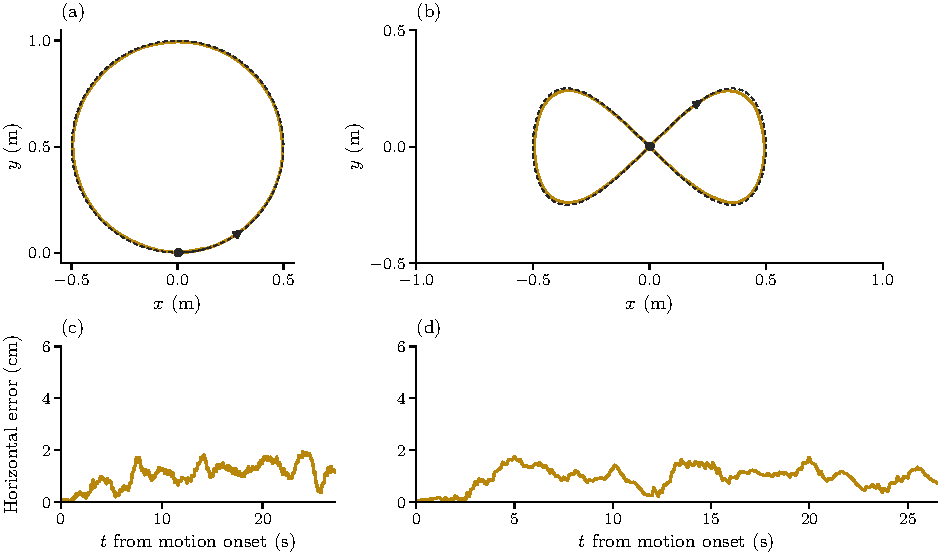
\includegraphics[width=\textwidth]{Images/trajectories.pdf}
\caption[The ring's path in the twin]{The ring's path in the rig twin at the rig's speed: three carriers, 0.125\,m/s
peak path speed, one run of each from the carry claim. (a) The orbit, one lap of radius 0.5\,m; (b) the figure-eight,
$a = 0.5$\,m. Gold: the ring's centre; dashed: the path; dot and arrow: start and direction. (c, d) The ring's
horizontal distance from the planner's reference, sampled at its 10\,Hz updates, from the onset of motion; this
time-indexed error includes the lag, which Table~\ref{tab:T7t} reports apart.}
\label{fig:traj}
\end{figure}

\subsubsection{The carry on the rig}
\label{sec:rig_results}

The hardware campaign covers carrying the ring with three and four UAVs and, since 7 October, releasing one UAV in
flight (Section~\ref{sec:res_leave}); the attach has not yet completed on the rig (Section~\ref{sec:res_join}). The
rig days, and what each changed, are in Appendix~\ref{sec:app_rig}. On 7 October four UAVs carried the ring on the
circle and the figure-eight, first on the planned rod pull and then with the trackers' measured pull and the rods
planned at 60$^\circ$ (Section~\ref{sec:tracker}; Table~\ref{tab:T7} and Figure~\ref{fig:F8}). Both paths flew about
three times closer to their references, the lags fell by half to two thirds, and the height's standard deviation fell from about 5 to
0.5\,cm. Six settings changed at once (Table~\ref{tab:T7}), so the table shows their combined effect: the measured pull alone flew the rods
at the planned 45$^\circ$, where a magnet let go 3.9\,s into the circle, and planning 60$^\circ$ keeps each magnet's
pull closer to its axis.

\begin{table}[htbp]
  \centering
  \footnotesize
  \caption[The carry on the rig]{The carry on the rig: four UAVs, the 0.86\,kg ring at 1.0\,m; the pull source and the
  rod plan against the path error. Error: the ring centre's horizontal distance from its reference from 4\,s into the
  path to LAND, mean and largest; lag: the time shift of the reference that minimises that error; height sd over the
  same window; one run each. K1 against K2 and K5 against K6 differ in six settings (pull source, planned and
  hand-over elevation, the pull cap, the landing unwind, the delay compensation): two configurations, not the pull
  source alone. [K3, K4 and K7: the next rig day.]}
  \label{tab:T7}
  \begin{tabularx}{\textwidth}{lYccYccc}
    \toprule
    Flight & Path & Pull source & Rod plan & Error mean / max (cm) & Lag (s) & Height sd (cm) & $n$ \\
    \midrule
    K1 & circle 0.125\,m/s & planned & 45$^\circ$ & 7.9 / 16.9 & 0.47 & 4.9 & 1 \\ % r006 (7 Oct); reviewer 12 Oct recomputed on this window; the registry row read 8.25 / 0.45 / 4.8 on the card's script
    K2 & circle 0.125\,m/s & measured & 60$^\circ$ & 2.6 / 5.5 & 0.17 & 0.5 & 1 \\ % r206e60; the registry's 2.91 / 0.20 are >10 % off on this window (reviewer): the R3 falsifier stays frozen on 2.91
    K3 & circle 0.125\,m/s & measured & 60$^\circ$ & [\dots] & [\dots] & [\dots] & [\dots] \\ % the repeat
    K4 & circle 0.125\,m/s & planned & 60$^\circ$ & [\dots] & [\dots] & [\dots] & [\dots] \\ % the falsifier
    K5 & figure-eight 0.25\,m/s & planned & 45$^\circ$ & 8.2 / 19.9 & 0.37 & 4.8 & 1 \\ % r0007; the registry's 0.41 s was a best shift too, its own row says 0.65 (along-track over speed)
    K6 & figure-eight 0.25\,m/s & measured & 60$^\circ$ & 2.9 / 6.6 & 0.19 & 0.6 & 1 \\ % r2008e60; registry 3.0 / 0.21 / 0.6
    K7 & hover 3 min & measured & 60$^\circ$ & [\dots] & -- & [\dots] & 1 \\ % the long hover
    \bottomrule
  \end{tabularx}
\end{table}

\begin{figure}[htbp]
\centering
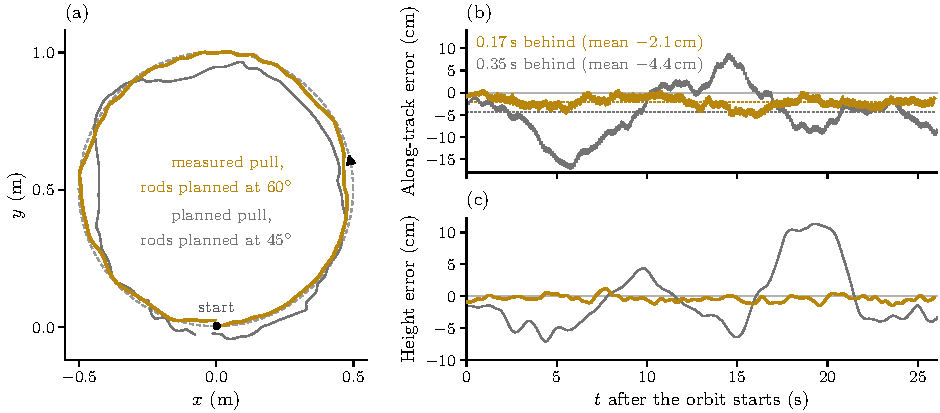
\includegraphics[width=\textwidth]{Images/rig_carry.pdf}
\caption[The circle on the rig: measured pull against planned pull]{The four-UAV circle on the rig, radius 0.5\,m at
0.125\,m/s, one lap: the trackers fed the rod pull they measure from motion capture with the rods planned at
60$^\circ$ (gold), against the same circle flown that morning on the planner's pull with the rods planned at
45$^\circ$ (grey); one run each. (a) Plan view of the ring's centre against the reference circle (dotted), with the
start and the direction of travel. (b) Along-track error, the ring's position along the circle minus the
reference's, negative behind; dotted: each run's mean, 2.1\,cm (0.17\,s) and 4.4\,cm (0.35\,s) behind, with the
worst 5.5 and 17\,cm. (c) Height error, measured minus planned, with a standard deviation of 0.5\,cm against
5.0\,cm.}
\label{fig:F8}
\end{figure}

\paragraph{The 60$^\circ$ planned-pull circle.} [Frozen falsifier, to score after the rig flies K4: if K4 lies within
max(1\,cm, the lap-to-lap sd of K3) of 2.91\,cm, the gain came from the rod angle, not the measurement. The 2.91\,cm
was frozen from the 7 October card's reading of K2; on this table's window the same flight reads 2.6\,cm, a
difference inside the 1\,cm tolerance.] In the twin (the even ring, two runs each, 0.09\,cm over the frozen floor) the planned
pull tracked the 60$^\circ$ circle better than the measured pull (Section~\ref{sec:res_levers}), so the twin does not
explain the rig's gain.
% 12 Oct: K1, K2, K5, K6 recomputed by the reviewer on one definition (window +4 s to LAND, lag by best time shift);
% the first-lap along-track numbers of fig:F8 (2.1 / 4.4 cm, 0.17 / 0.35 s) are a different window and are not these.

\subsubsection{Thrust identification}
\label{sec:thrust_id}

The 13 free hovers of Section~\ref{sec:tracker} fit
\begin{equation}
    u_T = a_i + 0.507\,M - 0.022\,(V - 23.5),
    \label{eq:thrust_fit}
\end{equation}
with $u_T$ the throttle, $M$ the mass carried (kg), $V$ the battery voltage and offsets $a_i$ of
0.181--0.187 for the four UAVs, with an rms residual of 0.003 (Figure~\ref{fig:thrust_map}). Above its
offset the map has a gain of 35.2\,m/s$^2$ per unit throttle for a 0.55\,kg UAV, which is the $k_T$ of
the tracker model \eqref{eq:trk_model}. With the map and one shared offset, the four UAVs hovered free
at +3.7, $-0.5$, $-0.4$ and +0.9\,cm from their targets with no integral action; the one 3.7\,cm high is
the UAV whose own offset is the lowest. A map identified at hover with one proportional gain had left
the UAVs 14--17\,cm low. Carrying the ring, the throttle the UAVs needed (0.55--0.60) matched what the
map predicted for their share of the load (0.569--0.575).

\begin{figure}[htbp]
\centering
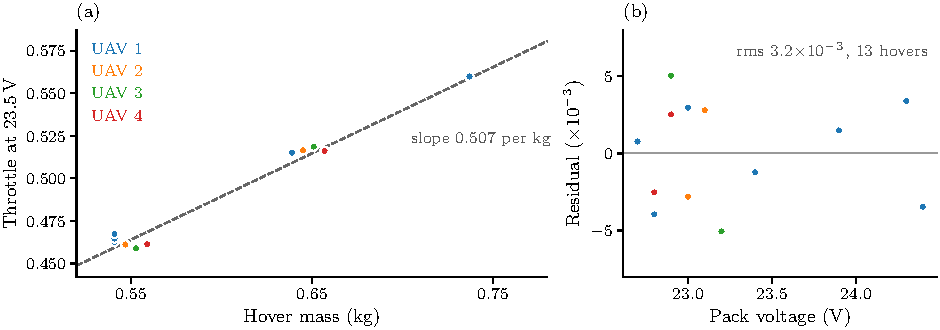
\includegraphics[width=\textwidth]{Images/thrust_map.pdf}
\caption[The rig's thrust map]{The rig's thrust map from 13 free hovers on 30 September, each UAV carrying 0, 98 or
196\,g. (a) Hover throttle corrected to 23.5\,V and to the mean offset, against the hover mass; one colour per UAV
(markers offset sideways by up to 9\,g so that hovers at the same mass can be seen); dashed: the fit
\eqref{eq:thrust_fit} with per-UAV offsets $a_i$ of 0.181--0.187. (b) The residuals of the fit against the pack
voltage: rms $3.2\times10^{-3}$, at most $5\times10^{-3}$ (about 1\,\% of hover throttle), with no trend left in
voltage.}
\label{fig:thrust_map}
\end{figure}

\subsubsection{Landing}
\label{sec:sim_landing}

Over the 82 landings of the freeze code tree in the rig twin (Table~\ref{tab:land}, Appendix~\ref{sec:app_tests}),
the unwind, the feedforward ramp and the ground idle kept every UAV within 0.65\,cm outside its reference and its lean
1.2\,s after touchdown at most 4.7$^\circ$ up to the moment the fleet was declared landed, where a straight descent pushed the UAVs 23.5\,cm outward. But 4 of the
82 landings disarmed the fleet with the UAVs still in the air, all four with one UAV stronger than its thrust map:
in three, every UAV was 0.46--0.53\,m up and fell onto its side. The stall test that declares touchdown had used up
its grace in the loaded descent, and when the ring touched down the strong UAV nearly held its height through the
second in which the UAVs blend to free hover, which read as a stall. With correct thrust maps on the rig's own
landing path (no unwind) the same fire came in 2 of 4 twin runs, at 0.42\,m. Re-arming the stall test at ring
touchdown (Section~\ref{sec:takeoff}) removed it in all 5 runs on that path and is now the twin's default; the rig
gets it after a review of its pose-freshness check. A UAV whose throttle offset is 0.03 below its map's (about 1\,m/s$^2$ of surplus thrust)
still stops about 16\,cm above its rest once the ring is down, is disarmed there and leans onto its rigid rod (Section~\ref{sec:discussion}); a
descent that keeps lowering its target for that case is under test.
% Sources: appendix re-fly (R2032, R2044, R2045 at 0.46-0.53 m; R2033 0.26 m; reviewer 17 Oct 02:40, C-L1 NOT
% supported); touchdown card re-fly (rig LAND path off 2 of 4: R2094, R2135; A 0 of 5: R2095, R2106, R2134, R2136,
% R2137; reviewer supported, twin default; must not say "ready for the rig"); residual 15.7-15.8 cm, 23.6-29.9 deg
% (R2088-R2091, R2099-R2102); land_descend_to_stall rev 3 flying 17-18 Oct (not thesis evidence yet).

\subsubsection{Computation}
\label{sec:res_compute}

Figure~\ref{fig:solve_time} gives the planner's optimisation time per tick in flight on the rig, 7--8
October, on the laptop that also runs the motion-capture and radio nodes. No tick of 7--8 October reached the 100\,ms tick. On
the rig days of 14--15 October, with three UAVs and the collaborator's stack running beside it, the planner solved in
31--46\,ms at the median and 46--65\,ms at the 95th percentile, with a slowest tick of 67--116\,ms. [The four-UAV median of 51--66\,ms against the rig's
60\,ms solve budget: to explain from the logs.] In the twin the stack solves 2--4 times slower than the solver alone,
under the load of the physics and the other nodes, but simulated time waits for the planner, so it always meets its
tick there. The 25 solve failures of the last rig flight of 30 September were traced to two faults acting together,
both now guarded (Appendix~\ref{sec:app_rig}).

\begin{figure}[htbp]
\centering
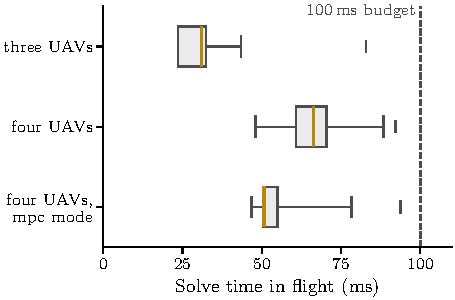
\includegraphics{Images/solve_time.pdf}
\caption[Planner solve time on the rig]{The planner's optimisation time in flight on the rig, 7--8 October:
three UAVs (after a detach, 15\,883 ticks), four UAVs (detach mode, 4\,762 ticks; carry mode, 22\,385 ticks). Box:
quartiles and median (gold); whiskers: 1st and 99th percentile; bar: the slowest tick. Medians 31, 66 and 51\,ms;
99th percentiles 44, 88 and 78\,ms; no tick reached the 100\,ms tick (dashed).}
\label{fig:solve_time}
\end{figure}

\paragraph{Answer to RQ1, the carry.} Yes, at lab speeds. On the rig four UAVs carried the ring around the circle
and through the figure-eight within 3\,cm of the path on average with the measured rod pull and the rods planned at
60$^\circ$, against about 8\,cm before (six settings changed together, so the measured pull alone is not yet
isolated); in the twin three UAVs carried it on five paths at peak path speeds up to 0.3\,m/s inside the frozen bars,
except the spin at 0.3\,m/s, and on 1\,m cables in the five cells flown up to 0.2\,m/s, with the ring running further
inside its curves as speed rises. A landing can still disarm a UAV in the air when its thrust
map is wrong: the re-armed touchdown test removes the 0.4--0.5\,m case in the twin, not the 16\,cm one, and the rig
does not have it yet.
